\documentclass[11pt]{article}
% * <emilgauti@gmail.com> 2018-02-17T15:23:17.915Z:
%
% ^.
\usepackage{amsmath,amssymb, amsthm, marvosym, permute, extsizes}
\usepackage{siunitx, graphicx, float, enumitem, adjustbox, hyperref, bm}
\usepackage{microtype, dsfont}
\usepackage[normalem]{ulem}
\usepackage[T1]{fontenc}
\usepackage[utf8]{inputenc}
\usepackage{lmodern}
\usepackage[T1]{fontenc}
\usepackage[a4paper,margin=2.5cm]{geometry}
\usepackage[icelandic]{babel}
\usepackage{minted}
\usemintedstyle{perldoc}
\usepackage{float}
\floatstyle{plaintop}
\restylefloat{table}
\parindent = 0pt

\title{Heimaverkefni 1\\ \vspace{0.4cm} \large Töluleg Greining}
\author{Emil Gauti Friðriksson,\\ Garðar Árni Skarphéðinsson,\\ Þorsteinn Jón Gautason}
\begin{document}
\maketitle % Mætti láta titil vera ofar á blaðinu svo við fáum pláss fyrir töflu 1 
\thispagestyle{empty}
\newpage
\setcounter{page}{1}
\section*{Dæmi 1}
Skrifið \texttt{Matlab} forrit sem hægt er að nota til að setja upp fylkið $A$ í (2.34). Notið síðan \texttt{Matlab} skipunina $\backslash$ í  til að leysa fyrir frávikin $y_i$ með $n = 10$.
\subsection*{Lausn}
Eftirfarandi forrit var notað til að setja upp fylkið $A$ úr (2.34) í bók.
\begin{minted}{matlab}
 %% Skilgreinum fylkið A
    A = zeros(n,n);
    A(1,:) = [16, -9, 8/3, -1/4, zeros(1, n-4)];
    A(2,:) = [-4, 6, -4, 1, zeros(1, n-4)];
    j = 0;
    for i = 3:n-2
        A(i,:) = [zeros(1,j), 1, -4, 6, -4, 1, zeros(1, n - (5 + j))]; 
        j = j + 1;
    end
    A(n-1,:) = [zeros(1,n-4), 1/17.*[16, -60, 72, -28]];
    A(n,:) = [zeros(1,n-4), 1/17.*[-12, 96, -156, 72]];
    A = sparse(A);
\end{minted}
Leysum síðan fyrir $y_i$ með $n=10$ fjölda skiptinga með forritinu {\mintinline{matlab}{LimpStick.m} (sjá \textbf{Forrit})
\begin{minted}{matlab}
%% Köllum á fallið til að fá reiknaða lausn y og rétta lausn g
    clear
    n = 10;
    [y, g,~,h] = LimpStick(n, 0, false);
\end{minted}
Þá fáum við:\\

\begin{table}[H]
\caption{Frávik brettis við lárétt}
\begin{center}
\begin{tabular}{l|l}
$i$		&  $y_i$	\\
\hline
1		&	-1.806$\cdot 10^4$		\\
2		&	-6.748$\cdot 10^4$		\\
3		&	-1.417$\cdot 10^3$		\\
4		&	-2.349$\cdot 10^3$		\\
5		&	-3.421$\cdot 10^3$		\\
6		&	-4.590$\cdot 10^3$		\\
7		&	-5.822$\cdot 10^3$		\\
8		&	-7.088$\cdot 10^3$		\\
9		&	-8.372$\cdot 10^3$		\\
10		&	-9.659$\cdot 10^3$		\\
\end{tabular}
\end{center}
\end{table}

\newpage
\section*{Dæmi 2}
Gerið graf með lausninni úr dæmi 1 ásamt réttu lausninni, gefin með formúlunni
\begin{align*}
	y(x)=\frac{f}{24EI}x^2(x^2-4Lx+6L^2)
\end{align*}
Þar sem $f$ er kraftur sem verkar á brettið vegna eigin þunga. Athugið skekkjuna í punktinum $x = L$.

\subsection*{Lausn}
Eftirfarandi graf sýnir reiknuðu lausnina úr \textbf{Dæmi 1} ásamt réttu lausninni. Notast var við $n=10$.

\begin{figure}[H]
\centering
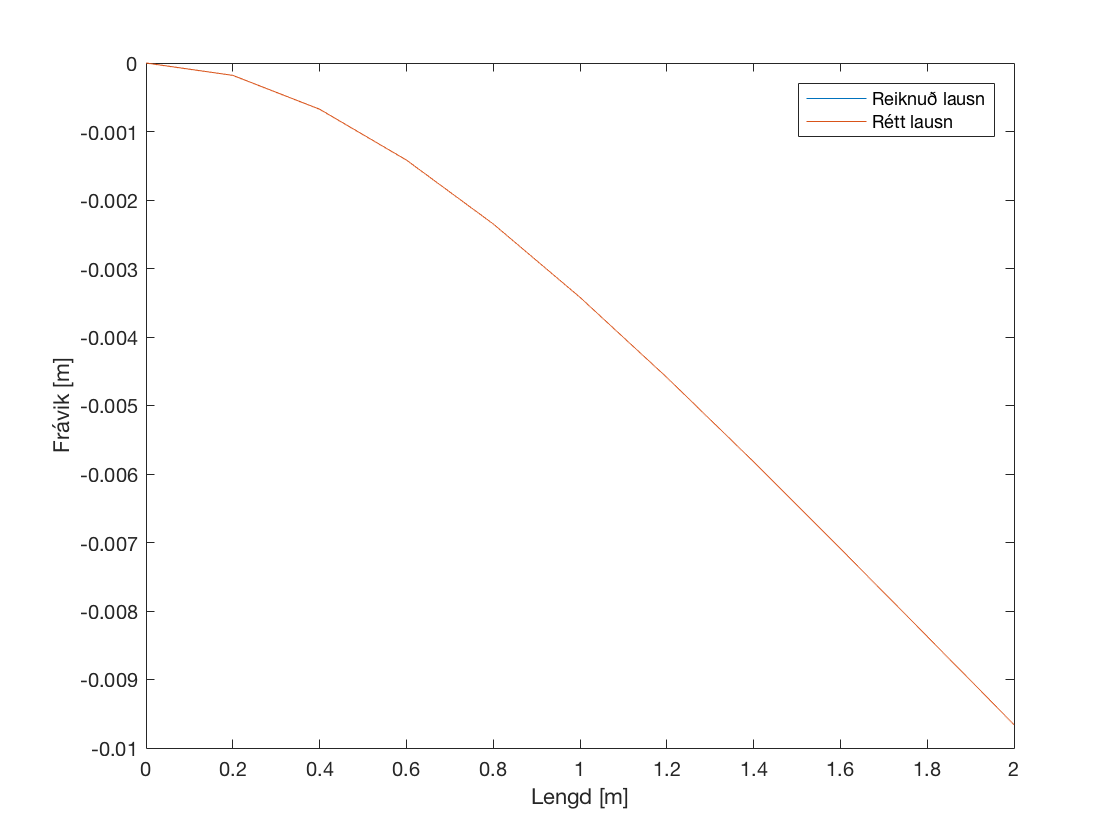
\includegraphics[scale=0.3]{bretti.png}
\caption{Stökkbretti undir eigin þyngd}
\end{figure}
Samkvæmt fyrirmælum er lengdin gefin með $L=\SI{2}{\meter}$ og skekkjan í þeim punkti er
\begin{minted}{matlab}
>> abs(g(n)-y(n))
ans =
     4.371503159461554e-16
\end{minted}
Sem er af sömu stærðargráðu og \texttt{eps}.


\newpage
\section*{Dæmi 3}

Keyrið reikningana úr \textbf{Dæmi 1} fyrir $n=10\cdot2^k$ þar sem $k=1,\dots,11$. Gerið töflu sem sýnir skekkjuna í $x = L$ fyrir öll $n$. Fyrir hvaða $n$ er skekkjan minnst? Hvers vegna byrjar skekkjan að aukast með $n$? Sniðugt er að gera aðra töflu fyrir ástandstölu fylkisins $A$ fyrir hvert $n$.

\subsection*{Lausn}

Keyrum reikningana úr \textbf{Dæmi 1} 11 sinnum, með $n = 10\cdot2^k$ fyrir $k = 1,\dots,11$ með eftirfarandi kóða:
\begin{minted}{matlab}
%% Endurtökum fyrir n = 10*2^k, k = 1:11
    clear
    err1 = zeros(1,11);
    cond1 = zeros(1,11);
    for k = 1:11
        n = 10*2^k;
        [y,g,A] = LimpStick(n, 0, false);
        err1(k) = abs(g(n)-y(n));
        cond1(k) = condest(A);
    end
\end{minted}
Þar sem notast er við fallið \texttt{condest()} til að reikna út gildi sparse fylkja. Gildin úr reikningunum má sjá í töflu 2.

\begin{table}[h!]
\caption{Skekkja og ástandstala fyrir breytilegt $n$}
\begin{center}
\begin{tabular}{l | l| l}
$n$ & Skekkja & Ástandstala\\
\hline
$10\cdot 2$			& 6.620$\cdot 10^{-15}$	& 5.303$\cdot 10^{5}$	\\
$10\cdot 2^2$		& 1.884$\cdot 10^{-13}$	& 8.449$\cdot 10^{6}$	\\
$10\cdot 2^3$		& 1.129$\cdot 10^{-12}$	& 1.348$\cdot 10^{8}$	\\
$10\cdot 2^4$		& 1.199$\cdot 10^{-11}$	& 2.154$\cdot 10^{9}$	\\
$10\cdot 2^5$		& 3.750$\cdot 10^{-10}$	& 3.443$\cdot 10^{10}$	\\
$10\cdot 2^6$		& 3.551$\cdot 10^{-10}$	& 5.507$\cdot 10^{11}$ \\
$10\cdot 2^7$		& 2.405$\cdot 10^{-9}$	& 8.810$\cdot 10^{12}$ \\    
$10\cdot 2^8$		& 1.551$\cdot 10^{-7}$	& 1.409$\cdot 10^{14}$	\\
$10\cdot 2^9$		& 3.737$\cdot 10^{-6}$	& 2.255$\cdot 10^{15}$	\\
$10\cdot 2^{10}$	& 3.936$\cdot 10^{-5}$	& 3.608$\cdot 10^{16}$	\\
$10\cdot 2^{11}$	& 5.006$\cdot 10^{-4}$	& 5.773$\cdot 10^{17}$	\\
\end{tabular}
\end{center}
\end{table}

Við sjáum út frá töflu 2 að $n=10\cdot 2$ hefur minnsta skekkju. Athugum einnig að skekkjan eykst með hækkandi $n$. Þetta er vegna þess að vídd fylkisins $A$ eykst með hækkandi $n$, sem hefur í för með sér vaxandi ástandstölu sem hefur áhrif á nákvæmni allra reikninga sem framkvæmdir eru með fylkinu.





\newpage
\section*{Dæmi 4}

Setjið bylgjulaga hrúgu á brettið. Þetta felur í sér að bæta liðnum $s(x) = -pg\sin\left(\frac{\pi}{L}x\right)$ við jöfnuna okkar fyrir $f(x)$. Sannið að jafnan

\begin{align*}
y(x)=\frac{f}{24EI}x^2(x^2-4Lx+6L^2)-\frac{pgL}{EI\pi}\left(\frac{L^3}{\pi ^3}\sin\left(\frac{\pi}{L}x\right)-\frac{x^3}{6}+\frac{L}{2}x^2-\frac{L^2}{\pi^2}x\right)
\end{align*}
uppfylli Euler-Bernoulli bjálkajöfnuna og jaðarskilyrðin fyrir fastan-frjálsan bjálka.
\subsection*{Lausn}

Jafnan:
\begin{align*}
y(x)=\frac{f}{24EI}x^2(x^2-4Lx+6L^2)-\frac{pgL}{EI\pi}\left(\frac{L^3}{\pi ^3}\sin\left(\frac{\pi}{L}x\right)-\frac{x^3}{6}+\frac{L}{2}x^2-\frac{L^2}{\pi^2}x\right)
\end{align*}

Þar sem $f$ er þyngdarkfraftur á lengdareiningu vegna brettisins sjálfs, á að vera rétta jafnan til þess að lýsa bognun brettisins þegar hrúgu með þyngdardreifingu $s(x)=-pg\sin\left(\frac{\pi}{L}x\right)$ er bætt ofan á brettið, og á hún því að uppfylla Euler-Bernoulli jöfnuna:

\begin{align*}
EIy^{(4)}=f(x)
\end{align*}

Þar sem $f(x)$ er heildar-þyngdarkraftur á lengdareiningu sem verkar á brettið. Eftir að framkvæma útreikningana fæst:

\begin{align*}
y^{(4)}=\frac{f}{EI}-\frac{pg}{EI}\sin\left(\frac{\pi}{L}x\right)
\end{align*}

Þ.e.a.s.

\begin{align*}
EIy^{(4)}=f-pg\sin\left(\frac{\pi}{L}x\right)=f+s(x)=f(x)
\end{align*}

Þar sem $s(x)$ er þyngdarkrafturinn á lengdareiningu vegna hrúgunnar ofan á brettinu. Til þess að vera alveg viss um að þetta standist þarf jafnan einnig að uppfylla jaðarskilyrðin sem fást frá því að brettið er fast í einn endann en frjálst í hinum. Þ.e.

\begin{align*}
y(0)=y'(0)=y''(L)=y'''(L)=0
\end{align*}

Setjum þessi gildi inn í afleiður $y(x)$ og fáum:

\begin{align*}y(0) &= \frac{f}{24EI}\cdot 0 -\frac{pgL}{EI\pi}\left(\frac{L^3}{\pi^3}\sin(0)-0\right)=0 \\
y'(0) &= \frac{f}{24EI}\cdot 0 -\frac{pgL}{EI\pi}\left(\frac{L^2}{\pi^2}\cos(0)-\frac{L^2}{\pi^2}\right)=0 \\
y''(L) &= \frac{f}{24EI}(12L^2-24L^2+12L^2)-\frac{pgL}{EI\pi}\left(-\frac{L}{\pi}\sin(\pi)-L+L\right)=0 \\
y'''(L) &= \frac{f}{24EI}(24L-24L)-\frac{pgL}{EI\pi}(-\cos(\pi)-1)=0
\end{align*}

Við sjáum því að jafnan uppfyllir skilyrðin fullkomlega.

\newpage
\section*{Dæmi 5}

Keyrið reikningana úr \textbf{Dæmi 3} fyrir bretti með bylgjulaga hrúgu. Setjið $p =\SI{100}{\kilo\gram}$ og gerið graf með reiknaðri lausn og réttri lausn. Svarið spurningunum úr \textbf{Dæmi 3} auk eftirfarandi spurningar: er skekkjan í $x = L$ í réttu hlutfalli við $h^2$?

\subsection*{Lausn}

Við framkvæmum sömu aðgerðir og í \textbf{Dæmi 3} fyrir tilfellið þar sem við höfum hrúguna úr \textbf{Dæmi 4} ofan á brettinu. Finnum þannig skekkjur og ástandstölur skv. þessum kóða:
\begin{minted}{matlab}
%% Eins of fyrri liðurinn, nema með hrúgu
    clf
    clear
    hold on
    err2 = zeros(1,11);
    hft1 = zeros(1,11);
    cond2 = zeros(1,11);
    [~,g,~,h] = LimpStick(10, 100, false);
    plot([0, h.*(1:10)], [0,g])
    for k = 1:11
        n = 10*2^k;
        [y,g,A,h] = LimpStick(n, 100, false);
        plot([0,h.*(1:n)], [0;y])
        err2(k) = abs(g(n) - y(n));
        cond2(k) = condest(A);
        hft1(k) = h;
    end
    hold off
\end{minted}

Fáum eftirfarandi niðurstöður:

\begin{table}[H]
\begin{center}
\caption{Skekkja og ástandstala fyrir breytilegt $n$}
\begin{tabular}{l | l| l}
$n$ & Skekkja & Ástandstala\\
\hline
$10\cdot 2$			& 5.377$\cdot 10^{-4}$	& 5.303$\cdot 10^{5}$	\\
$10\cdot 2^2$		& 1.355$\cdot 10^{-4}$	& 8.449$\cdot 10^{6}$	\\
$10\cdot 2^3$		& 3.393$\cdot 10^{-5}$	& 1.348$\cdot 10^{8}$	\\
$10\cdot 2^4$		& 8.487$\cdot 10^{-6}$	& 2.154$\cdot 10^{9}$	\\
$10\cdot 2^5$		& 2.120$\cdot 10^{-6}$	& 3.443$\cdot 10^{10}$	\\
$10\cdot 2^6$		& 5.429$\cdot 10^{-7}$	& 5.507$\cdot 10^{11}$ \\
$10\cdot 2^7$		& 4.591$\cdot 10^{-7}$	& 8.810$\cdot 10^{12}$ \\    
$10\cdot 2^8$		& 1.479$\cdot 10^{-6}$	& 1.409$\cdot 10^{14}$	\\
$10\cdot 2^9$		& 2.324$\cdot 10^{-5}$	& 2.255$\cdot 10^{15}$	\\
$10\cdot 2^{10}$	& 6.619$\cdot 10^{-4}$	& 3.608$\cdot 10^{16}$	\\
$10\cdot 2^{11}$	& 7.052$\cdot 10^{-4}$	& 5.773$\cdot 10^{17}$	\\
\end{tabular}
\end{center}
\end{table}
\newpage
Teiknum gröf fyrir sérhver gildi á $k$:
\begin{figure}[H]
\centering
  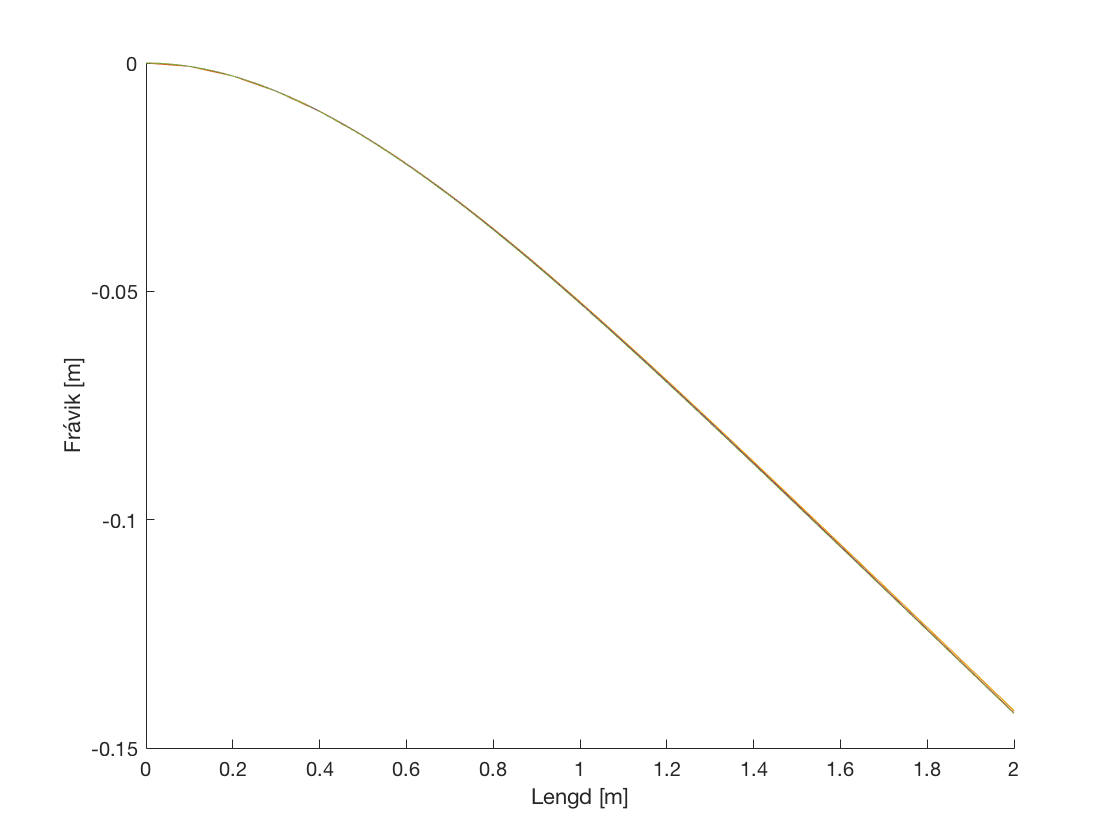
\includegraphics[width=5in]{bretti_m_hrugu.png}
  \caption{Bretti með hrúgu}
\end{figure}
\begin{figure}[H]
\centering
  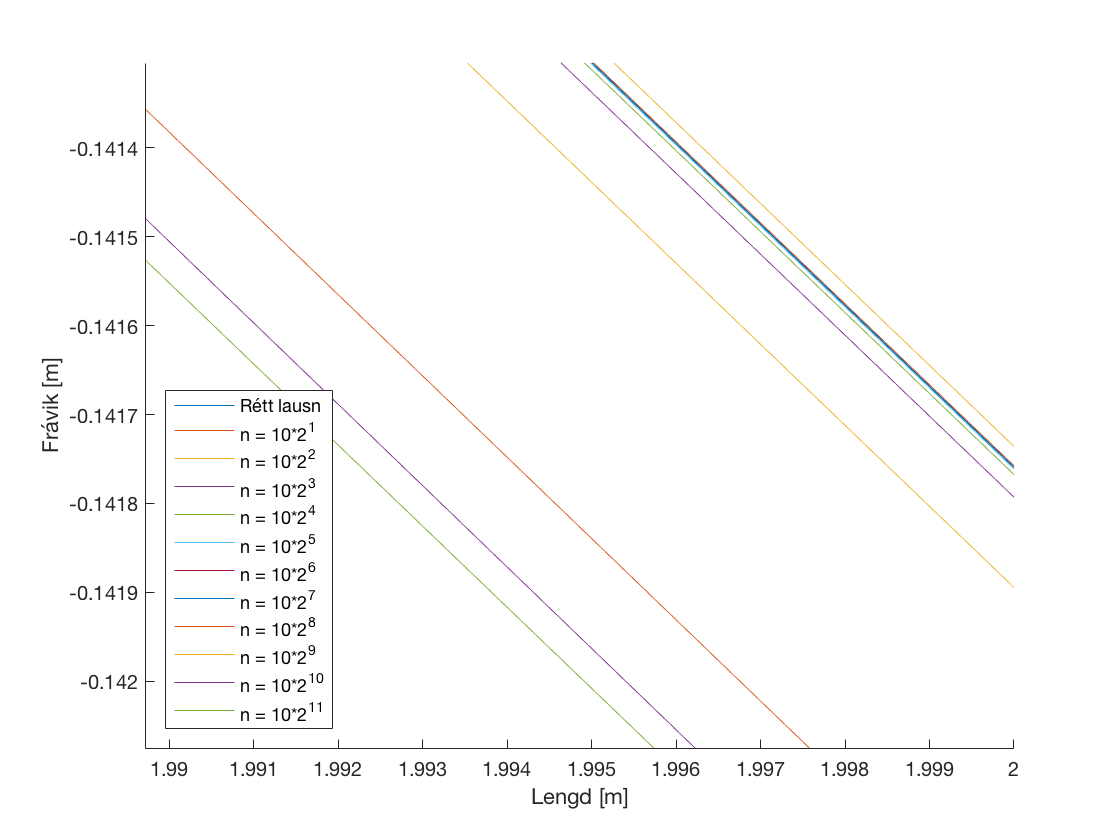
\includegraphics[width=5in]{m_hrugu_close.png}
\caption{Bretti með hrúgu (nærmynd)}
\end{figure}
\newpage
Við sjáum að þessar niðurstöður eru frábrugðnar þeim úr \textbf{Dæmi 3}. Það er ekkert augljóst samband á milli skekkjunnar og $h^2$. Við sjáum einnig að með hækkandi $n$ minnkar skekkjan til að byrja með en byrjar að hækka aftur eftir $n=10\cdot 2^7$ þrátt fyrir að ástandstalan haldi bara áfram að hækka.\\
\begin{figure}[H]
\centering
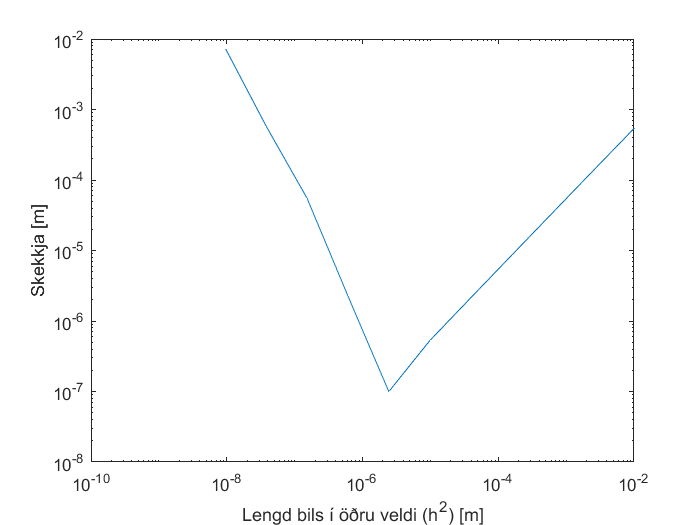
\includegraphics[scale=0.64]{loglogGraf_5_.png}
\caption{log-log graf af skekkju sem falli af $h^2$}
\end{figure}
\newpage
\section*{Dæmi 6}

Fjarlægið hrúguna af brettinu og bætið við \SI{70}{\kilo\gram} dýfingarmanni á seinustu \SI{20}{\centi\meter} af brettinu. Þið verðið að bæta viðeigandi lið við kraftajöfnuna $f(x)$. Reiknið frávik brettisins í punktinum $x = L$ fyrir æskilegt gildi $n$ úr \textbf{Dæmi 5} og gerið graf af lausninni.

\subsection*{Lausn}

Framkvæmum sömu útreikninga og í \textbf{Dæmi 2} fyrir tilfellið þar sem dýfingarmaður stendur á enda brettisins, $1.8m\leq x_i \leq 2m$, með $n=10 \cdot 2^7$ skv. eftirfarandi kóða:
\begin{minted}{matlab}
%% Eins og fyrri liðurinn, nema með dýfingarmanni
    clear
    clf
    n = 10*2^7;
    [y,~,~,h] = LimpStick(n, 0, true);
    plot([0, h*(1:n)], [0; y])
    def = y(n);
    ylabel("Frávik [m]")
    xlabel("Lengd [m]")
\end{minted}
Teiknum graf:\\
\begin{figure}[h!]
\centering
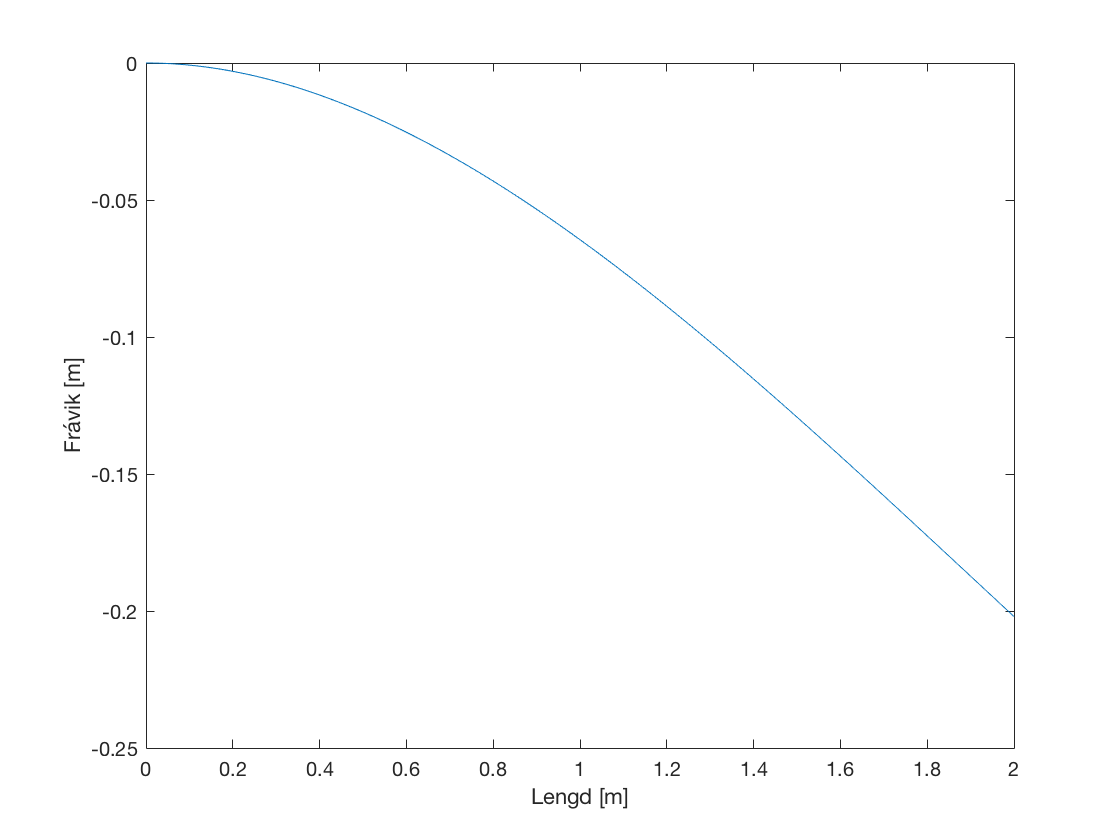
\includegraphics[scale=0.32]{bretti_m_dyfingarmanni.png}
\caption{Stökkbretti með dýfingarmanni}
\end{figure}

\newpage
\section*{Dæmi 7}

Festum nú báða enda brettisins og bætum hrúgunni aftur ofan á. Þörf er á breytingum á fylkinu $A$. Reiknið frávik fyrir bylgjulaga hrúgu og reiknið skekkjuna í punktinum $x = L/2$. Rétt lausn fæst með formúlunni
\begin{align*}
	y(x) = \frac{f}{24EI}x^2(L-x)^2 - \frac{pgL^2}{\pi^4EI}\left(L^2\sin\left(\frac{\pi}{L}x\right) + \pi x(x - L)\right)
\end{align*}

\subsection*{Lausn}
Skoðum nú hvað gerist þegar brettið er fest í báða enda og hrúgan úr \textbf{Dæmi 5} er aftur sett ofan á það. Við gerum þetta með kóðanum: 
\begin{minted}{matlab}
%% Festum planka í báða enda
    clf
    clear
    hold on
    err3 = zeros(1,11);
    hft2 = zeros(1,11);
    cond3 = zeros(1,11);
    [~,g,~,h] = LimpBridge(10, 100);
    plot([0, h.*(1:10)], [0,g])
    for k = 1:11
        n = 10*2^k;
        [y,g,A,h] = LimpBridge(n, 100);
        plot([0,h.*(1:n)], [0;y])
        err3(k) = abs(y(round(n/2)) - g(round(n/2)));
        cond3(k) = condest(A);
        hft2(k) = h;
    end
    axis([0,2, -0.02, 0.02])
    hold off
\end{minted}

Framkvæmum sömu aðgerðir og í \textbf{Dæmi 5} í punktinum $x=L/2$ og setjum niðurstöðurnar upp í töflu:
\begin{table}[h]
\caption{Skekkja og ástandstala fyrir breytilegt $n$}
\begin{center}
\begin{tabular}{l | l| l}
$n$ & Skekkja & Ástandstala\\
\hline
$10\cdot 2$			& 1.465$\cdot 10^{-5}$	& 1.065$\cdot 10^{4}$\\
$10\cdot 2^2$		& 3.853$\cdot 10^{-6}$	& 1.546$\cdot 10^{5}$\\
$10\cdot 2^3$		& 9.878$\cdot 10^{-7}$	& 2.354$\cdot 10^{6}$\\
$10\cdot 2^4$		& 2.501$\cdot 10^{-7}$	& 3.675$\cdot 10^{7}$\\
$10\cdot 2^5$		& 6.291$\cdot 10^{-8}$	& 5.806$\cdot 10^{8}$\\
$10\cdot 2^6$		& 1.578$\cdot 10^{-8}$	& 9.233$\cdot 10^{9}$\\
$10\cdot 2^7$		& 3.834$\cdot 10^{-9}$	& 1.473$\cdot 10^{11}$\\    
$10\cdot 2^8$		& 1.901$\cdot 10^{-9}$	& 2.352$\cdot 10^{12}$\\
$10\cdot 2^9$		& 8.534$\cdot 10^{-9}$	& 3.761$\cdot 10^{13}$\\
$10\cdot 2^{10}$	& 3.503$\cdot 10^{-7}$	& 6.016$\cdot 10^{14}$\\
$10\cdot 2^{11}$	& 6.905$\cdot 10^{-6}$	& 9.616$\cdot 10^{15}$\\
\end{tabular}
\end{center}
\end{table}
Fáum einnig eftirfarandi myndir:
\begin{figure}[H]
\centering
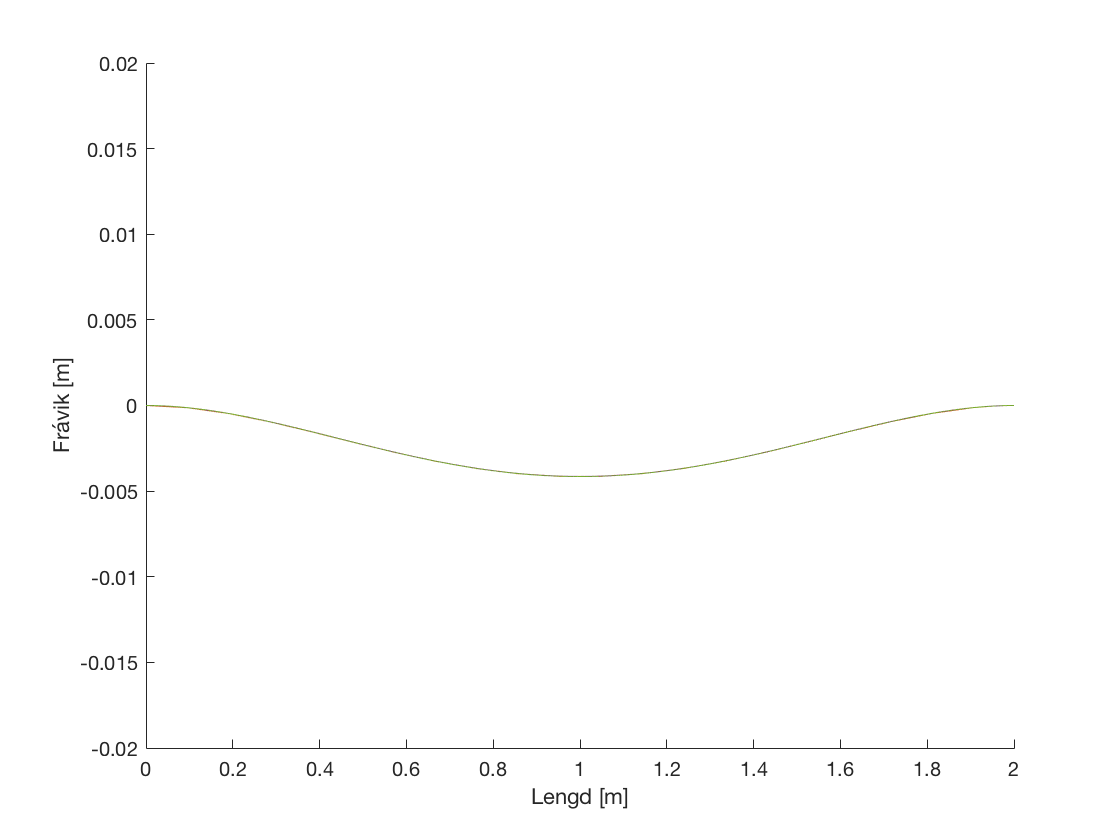
\includegraphics[scale=0.3]{britch.png}
\caption{Bretti fest í báða enda}
\end{figure}
\begin{figure}[H]
\centering
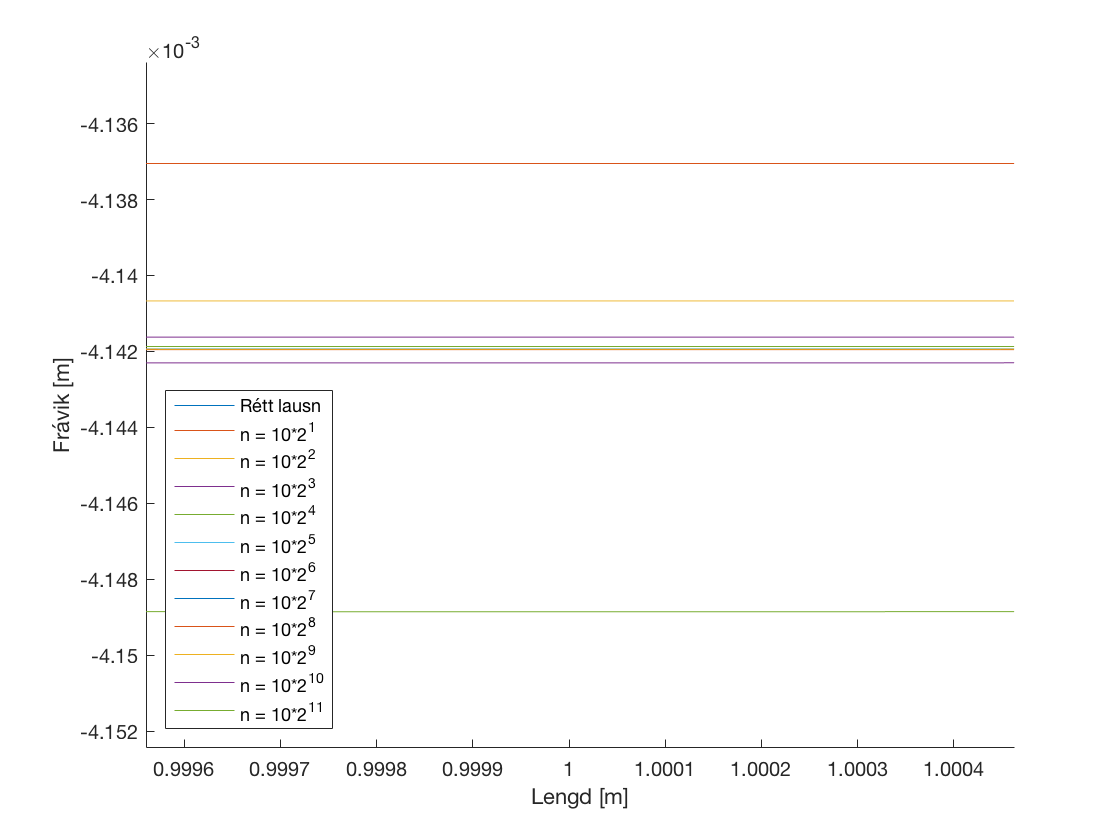
\includegraphics[scale=0.3]{britch_close.png}
\caption{Bretti fest í báða enda (nærmynd)}
\end{figure}








\newpage
\section*{Dæmi 8}

Hér eru gefnar hugmyndir um frekari tilraunir á mismunandi brettum með mismunandi breidd, þykkt og gerð. Framkvæmið nokkra reikninga sem svara til mismunandi bretta.

\subsection*{Lausn}

Við ætlum að bera saman venjulegt bretti, bretti með tvöfalda breidd og þykkt, auk rör- og sívalningslaga brettis með sama þverskurðarflatarmál og venjulega brettið. Síðan athugum við sveigjuna á þessum brettum miðað við tvöfalt venjulegt bretti. 

\begin{figure}[H]
\begin{center}
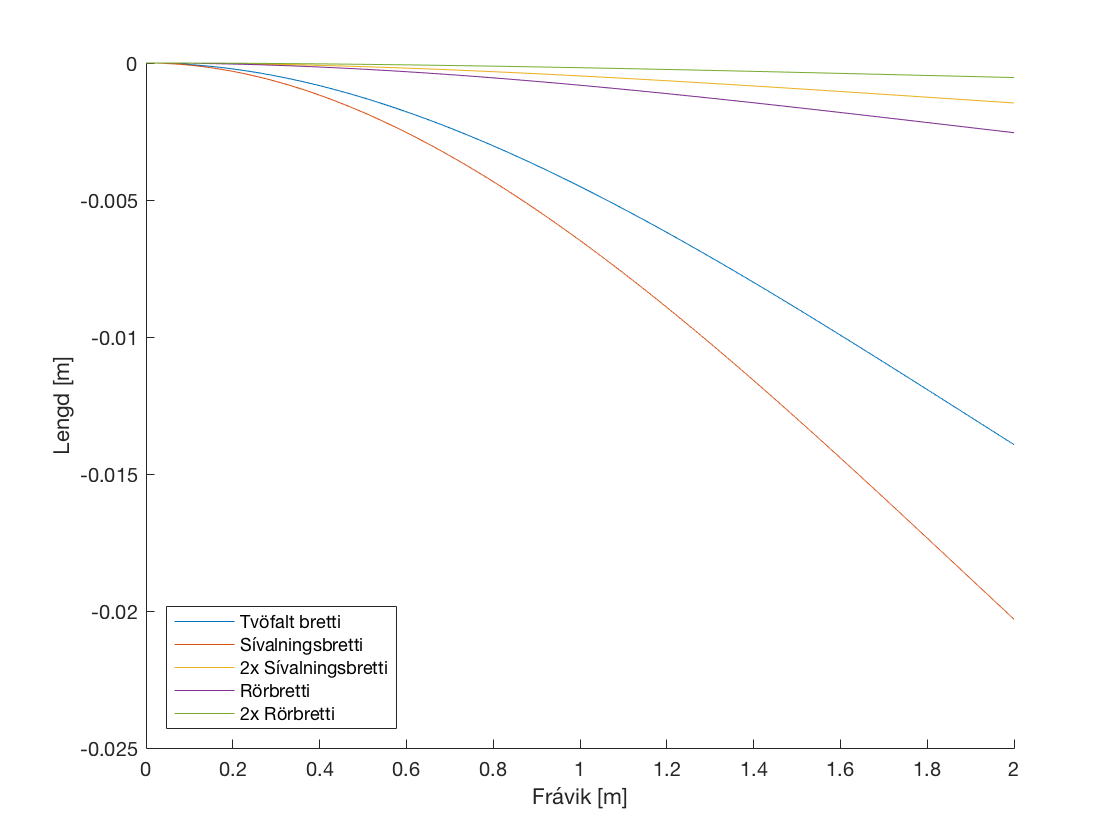
\includegraphics[scale=0.26]{hellingur.png}
\caption{Mismunandi gerðir bretta}
\end{center}
\end{figure}

Einnig könnum við sveigju brettis sem er gert úr Jello{\texttrademark} og gulli með mismunandi þykktir. Gerum graf sem sýnir frávik frá láréttu sem fall af fjarlægð fyrir efnin tvö.
\begin{figure}[H]
\centering
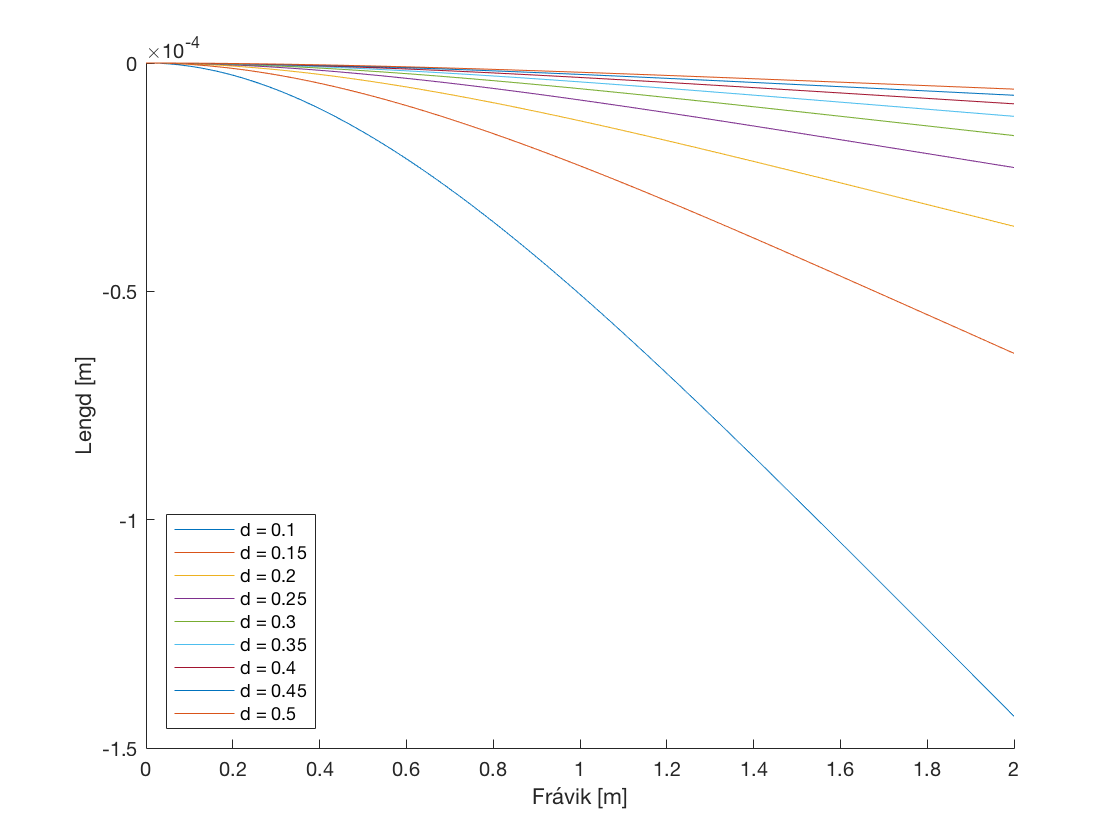
\includegraphics[scale=0.3]{gullstick.png}
\caption{Bretti úr gulli fest í annan endann}
\end{figure}
\begin{figure}[H]
\centering
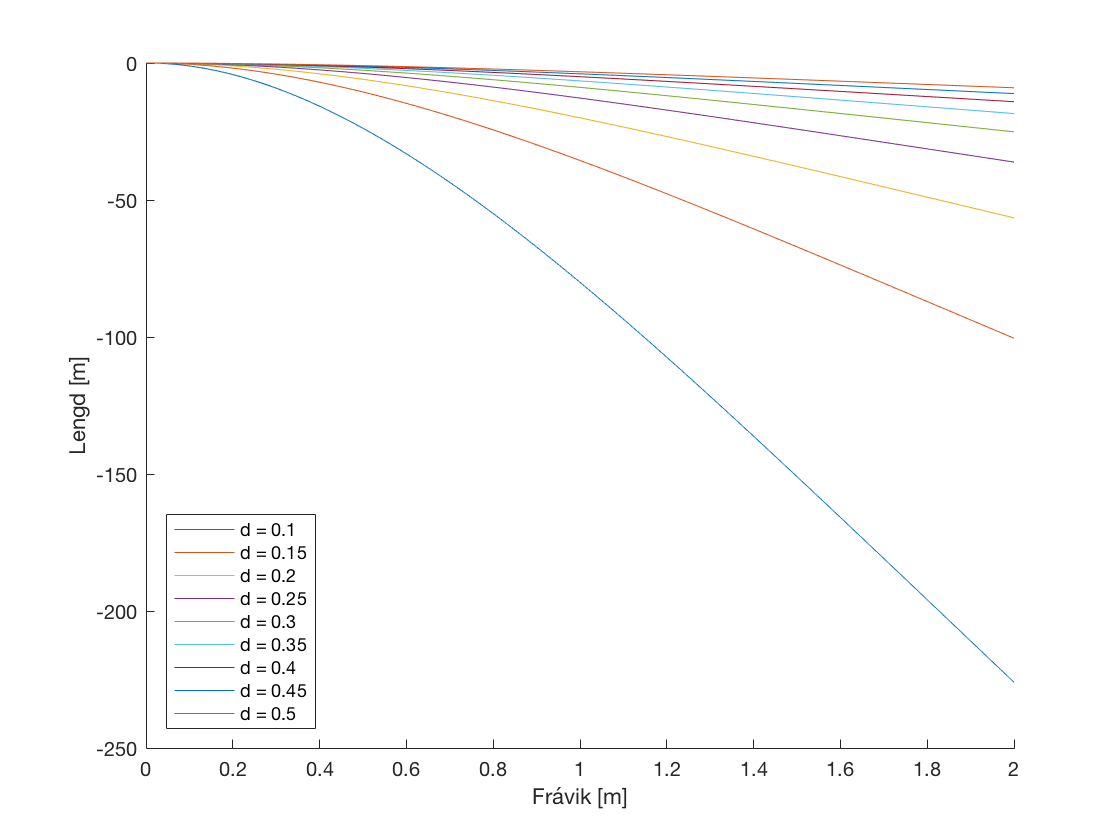
\includegraphics[scale=0.3]{jello.png}
\caption{Bretti úr Jello{\texttrademark} fest í annan endann}
\end{figure}
Athugum að reikniaðferðin sem notast var við gerir ekki ráð fyrir fastri lengd á bretti eins og sést greinilega á mynd 10.










\newpage
\section*{Forrit}


\section*{\mintinline{matlab}{LimpStick.m}}
\begin{minted}{matlab}
function [y, g, A, h] = LimpStick(n, p, diver)
%LimpStick reiknar út frávik stökkbrettis frá jafnvægisstöðu.
%   Úttök LimpStick eru reiknað frávik y, nákvæmt frávik g, 
%   fylkið A og lengd bilanna, h.
%   Inntök LimpStick er fjöldi bila n, þyngd hrúgu p, og rökgildið
%   diver, sem segir til um hvort dýfingarmaður sé á brettinu eða ekki.
%
%See also LIMPBRIDGE, LIMPSTICK8.
    
    %% Skilgreinum fasta
    L = 2;
    h = L/n;
    E = 1.3e10;
    w = 0.3;
    d = 0.03;
    I = w*d^3/12;
    g = -9.81;
    CTE = h^4/(E*I);
    %% Skilgreinum fylkið A
    A = zeros(n,n);
    A(1,:) = [16, -9, 8/3, -1/4, zeros(1, n-4)];
    A(2,:) = [-4, 6, -4, 1, zeros(1, n-4)];
    j = 0;
    for i = 3:n-2
        A(i,:) = [zeros(1,j), 1, -4, 6, -4, 1, zeros(1, n - (5 + j))]; 
        j = j + 1;
    end
    A(n-1,:) = [zeros(1,n-4), 1/17.*[16, -60, 72, -28]];
    A(n,:) = [zeros(1,n-4), 1/17.*[-12, 96, -156, 72]];
    A = sparse(A);
    %% Skilgreinum vigurinn f
    % Tekið er tillit til þyngdar hrúgu og/eða dýfingarmanns.
    f = zeros(n,1);
    for i = 1:n
        if diver
            if h*i > 1.8
                f(i) = 480*w*d*g + p*g*sin(h*i*pi/L) + g*70/0.2;
            else
                f(i) = 480*w*d*g + p*g*sin(h*i*pi/L);
            end
        else
            f(i) = 480*w*d*g + p*g*sin(h*i*pi/L);
        end
    end
    y = A\(CTE*f);
    %% Skilgreinum réttu lausnina
    %Rétt lausn er reiknuð með sama fjölda bila og reiknaða lausnin.
    p = @(x) ((480*w*d*g)/(24*E*I))*x^2*(x^2 - 4*L*x + 6*L^2) 
    + (p*g*L/(E*I*pi))*(L^3/pi^3*sin(pi/L*x) - x^3/6 + L/2*x^2 - L^2/pi^2*x);
    g = zeros(1,n);
    for i = 1:n
        j = h*i;
        g(i) = p(j);
    end
end
\end{minted}
\newpage

\section*{\mintinline{matlab}{ToluBois.m}}
\begin{minted}{matlab}
%% Köllum á fallið til að fá reiknaða lausn y og rétta lausn g
    clear
    n = 10;
    [y, g,~,h] = LimpStick(n, 0, false);
    plot([0,h.*(1:n)], [0;y])
    hold on
    plot([0, h.*(1:n)], [0,g])
    xlabel("Lengd [m]");
    ylabel("Frávik [m]");
    legend("Reiknuð lausn", "Rétt lausn");
    hold off
    format long
    skekkja = abs(g(n)-y(n));
%% Endurtökum fyrir n = 10*2^k, k = 1:11
    clear
    err1 = zeros(1,11);
    cond1 = zeros(1,11);
    hft0 = zeros(1,11);
    for k = 1:11
        n = 10*2^k;
        [y,g,A,h] = LimpStick(n, 0, false);
        err1(k) = abs(g(n)-y(n));
        cond1(k) = condest(A);
        hft0(k) = h;
    end
%% Eins of fyrri liðurinn, nema með hrúgu
    clf
    clear
    hold on
    err2 = zeros(1,11);
    hft1 = zeros(1,11);
    cond2 = zeros(1,11);
    [~,g,~,h] = LimpStick(1000, 100, false);
    plot([0, h.*(1:1000)], [0,g])
    for k = 1:11
        n = 10*2^k;
        [y,g,A,h] = LimpStick(n, 100, false);
        plot([0,h.*(1:n)], [0;y])
        err2(k) = abs(g(n) - y(n));
        cond2(k) = condest(A);
        hft1(k) = h;
    end
    %axis([0, 2.1, -0.2, 0])
    legend("Rétt lausn", "n = 10*2^1", "n = 10*2^2", "n = 10*2^3", "n = 10*2^4", 
    "n = 10*2^5", "n = 10*2^6", "n = 10*2^7", "n = 10*2^8", "n = 10*2^9", "n = 10*2^{10}", 
    "n = 10*2^{11}", "Interpreter", "latex", "Location", "southwest");
    ylabel("Frávik [m]");
    xlabel("Lengd [m]");
    %title("Stökkbretti með samhverfri hrúgu");
    hold off
%% Eins og fyrri liðurinn, nema með dýfingarmanni
    clear
    clf
    n = 10*2^7;
    [y,~,~,h] = LimpStick(n, 0, true);
    plot([0, h*(1:n)], [0; y])
    def = y(n);
    ylabel("Frávik [m]")
    xlabel("Lengd [m]")
%% Festum planka í báða enda
    clf
    clear
    hold on
    err3 = zeros(1,11);
    hft2 = zeros(1,11);
    cond3 = zeros(1,11);
    [~,g,~,h] = LimpBridge(10000, 100);
    plot([0, h.*(1:10000)], [0,g])
    for k = 1:11
        n = 10*2^k;
        [y,g,A,h] = LimpBridge(n, 100);
        plot([0,h.*(1:n)], [0;y])
        err3(k) = abs(y(round(n/2)) - g(round(n/2)));
        cond3(k) = condest(A);
        hft2(k) = h;
    end
    axis([0,2, -0.02, 0.02])
    ylabel("Frávik [m]")
    xlabel("Lengd [m]")
    legend("Rétt lausn", "n = 10*2^1", "n = 10*2^2", "n = 10*2^3", "n = 10*2^4", 
    "n = 10*2^5", "n = 10*2^6", "n = 10*2^7", "n = 10*2^8", "n = 10*2^9", "n = 10*2^{10}", 
    "n = 10*2^{11}", "Interpreter", "latex", "Location", "southwest");
    hold off
%% Allar myndir saman
    clear
    clf
    hold on
    n = 10*2^7;
    [y, ~,~,h] = LimpStick(n, 0, false);
    plot([0,h.*(1:n)], [0;y])
    [y,~,~,~] = LimpStick(n, 100, false);
    plot([0,h.*(1:n)], [0;y])
    [y,~,~,~] = LimpStick(n, 0, true);
    plot([0, h*(1:n)], [0; y])
    ylabel("Frávik [m]")
    xlabel("Lengd [m]")
\end{minted}

\newpage
\section*{\mintinline{matlab}{LimpBridge.m}}
\begin{minted}{matlab}
function [y,g,A,h] = LimpBridge(n, p)
% LimpBridge reiknar frávik brúar frá jafnvægisstöðu undir álagi frá hrúgu
% með þyngd p.
%   LimpBridge tekur inn fjölda bila n og þyngd hrúgu p.
%   LimpBridge skilar reiknuðu fráviki y, nákvæmu fráviki g, fylkinu A og
%   lengd bila h.
%See also LIMPSTICK, LIMPSTICK8.

    %% Skilgreinum fasta
    L = 2;
    h = L/(n + 1);
    E = 1.3e10;
    w = 0.3;
    d = 0.03;
    I = w*d^3/12;
    g = -9.81;
    CTE = h^4/(E*I);
    %% Skilgreinum fylkið A
    A = zeros(n,n);
    A(1,:) = [16, -9, 8/3, -1/4, zeros(1, n-4)];
    A(2,:) = [-4, 6, -4, 1, zeros(1, n-4)];
    j = 0;
    for i = 3:n-2
        A(i,:) = [zeros(1,j), 1, -4, 6, -4, 1, zeros(1, n - (5 + j))]; 
        j = j + 1;
    end
    A(n-1,:) = fliplr(A(2,:));
    A(n,:) = fliplr(A(1,:));
    A = sparse(A);
    %% Skilgreinum vigurinn f
    f = zeros(n,1);
    for i = 1:n
        f(i) = 480*w*d*g + p*g*sin(h*i*pi/L);
    end
    %% Reiknum lausn
    y = A\(f*CTE);
    %% Skilgreinum nákvæma lausn
    p = @(x) ((480*w*d*g)/(24*E*I))*x^2*(L-x)^2 + (p*g*L^2/(pi^4*E*I))*(L^2*sin(pi*x/L) 
    + pi*x*(x - L));
    g = zeros(1,n);
    for i = 1:n
        j = h*i;
        g(i) = p(j);
    end
end
\end{minted}

\newpage
\section*{\mintinline{matlab}{LimpStick8.m}}
\begin{minted}{matlab}
function [y, g, A, h] = LimpStick8(n,w,d,p,diver,shape, E)
%LimpStick8 reiknar út frávik stökkbrettis frá jafnvægisstöðu, en ræður við
%mismunandi gerðir bretta.
%   LimpStick8 tekur inn fjölda bila n, breidd brettis w, þykkt brettis d,
%   þyngd hrúgu p, rökgildið diver, breytuna shape sem segir til um gerð
%   brettis og Young's modulus tiltekins efnis, E.
%   k er kassalaga bretti með þykkt d og breidd w
%   h er sívalningslaga bretti með sama flatarmál og kassalaga brettið.
%   g er rörlaga bretti með fastan 10cm radíus en annars sama flatarmál og
%   kassalaga brettið.

    %% Skilgreinum fasta
    L = 2;
    h = L/n;
    if shape == 'k'
        I = w*d^3/12;
    elseif shape == 'h'
        I = pi*(sqrt(w*d/pi))^4/4;
    elseif shape == 'g'
        %gefum okkur innri radíus 10cm
        I = pi*(sqrt(w*d/pi + 0.1^2)^4 - 0.1^4)/4;
    end
    g = -9.81;
    CTE = h^4/(E*I);
    %% Skilgreinum fylkið A
    A = zeros(n,n);
    A(1,:) = [16, -9, 8/3, -1/4, zeros(1, n-4)];
    A(2,:) = [-4, 6, -4, 1, zeros(1, n-4)];
    j = 0;
    for i = 3:n-2
        A(i,:) = [zeros(1,j), 1, -4, 6, -4, 1, zeros(1, n - (5 + j))]; 
        j = j + 1;
    end
    A(n-1,:) = [zeros(1,n-4), 1/17.*[16, -60, 72, -28]];
    A(n,:) = [zeros(1,n-4), 1/17.*[-12, 96, -156, 72]];
    A = sparse(A);
    %% Skilgreinum vigurinn f
    f = zeros(n,1);
    for i = 1:n
        if diver
            if h*i > 1.8
                f(i) = 480*w*d*g + p*g*sin(h*i*pi/L) + g*70/0.2;
            else
                f(i) = 480*w*d*g + p*g*sin(h*i*pi/L);
            end
        else
            f(i) = 480*w*d*g + p*g*sin(h*i*pi/L);
        end
    end
    y = A\(CTE*f);
    %% Skilgreinum réttu lausnina
    p = @(x) ((480*w*d*g)/(24*E*I))*x^2*(x^2 - 4*L*x + 6*L^2) 
    + (p*g*L/(E*I*pi))*(L^3/pi^3*sin(pi/L*x) - x^3/6 + L/2*x^2 - L^2/pi^2*x);
    g = zeros(1,n);
    for i = 1:n
        j = h*i;
        g(i) = p(j);
    end
end
\end{minted}

\newpage
\section*{\mintinline{matlab}{pt8.m}}
\begin{minted}{matlab}
n = 100;
w = 0.3;
d = 0.03;
y = zeros(6,n+1);
g = y;
deflection = zeros(1,6);

[y1, g1,~,h] = LimpStick8(n, w, d, 0, true, 'k', 1.3e10);
    y(1,:) = [0, y1.'];
    g(1,:) = [0, g1];
[y2, g2,~,~] = LimpStick8(n, 2*w, 2*d, 0, true, 'k', 1.3e10);
    y(2,:) = [0, y2.'];
    g(2,:) = [0, g2];
[y3, g3,~,~] = LimpStick8(n, w, d, 0, true, 'h', 1.3e10);
    y(3,:) = [0, y3.'];
    g(3,:) = [0, g3];
[y4, g4,~,~] = LimpStick8(n, 2*w, 2*d, 0, true, 'h', 1.3e10);
    y(4,:) = [0, y4.'];
    g(4,:) = [0, g4];
[y5, g5,~,~] = LimpStick8(n, w, d, 0, true, 'g', 1.3e10);
    y(5,:) = [0, y5.'];
    g(5,:) = [0, g5];
[y6, g6,~,~] = LimpStick8(n, 2*w, 2*d, 0, true, 'g', 1.3e10);
    y(6,:) = [0, y6.'];
    g(6,:) = [0, g6];

hold on

titlar = {'Bretti', 'Tvöfalt bretti', 'Sívalningur', 'Tvöfaldur sívalningur', 
'Rör með innri radíus 10cm', 'Tvöfalt rör með innri radíus 10cm'};

for i = 1:6
    subplot(2,3,i);
    plot([0,h.*(1:n)], y(i,:));
    title(titlar(i));
    xlabel("Frávik [m]");
    ylabel("Lengd [m]");
    deflection(i) = y(i,n+1);
end


%% Jello sticks
% G.r.f. Young's stuðli 50kPa.
clf
clear
n = 1000;
hold on
for d = 0.1:0.05:0.5
    [y,g,~,h] = LimpStick8(n,0.5,d,0,false,'k',50000);
    plot([0,h.*(1:1000)],[0;y])
end
xlabel("Frávik [m]");
ylabel("Lengd [m]");
legend("d = 0.1", "d = 0.15", "d = 0.2", "d = 0.25", "d = 0.3", "d = 0.35", 
"d = 0.4", "d = 0.45", "d = 0.5", "Location", "southwest");
hold off
%% Gull
clf
clear
n = 1000;
hold on
for d = 0.1:0.05:0.5
    [y,g,~,h] = LimpStick8(n,0.5,d,0,false,'k',79e9);
    plot([0,h.*(1:1000)],[0;y])
end
xlabel("Frávik [m]");
ylabel("Lengd [m]");
legend("d = 0.1", "d = 0.15", "d = 0.2", "d = 0.25", "d = 0.3", "d = 0.35", 
"d = 0.4", "d = 0.45", "d = 0.5", "Location", "southwest");
hold off


\end{minted}


\mbox{}
\vfill
\begin{tabular}[b]{c c c}
& & \\[8ex]
\makebox[2in]{\hrulefill} & \makebox[2in]{\hrulefill} & \makebox[2in]{\hrulefill}\\[6ex]
Þorsteinn Jón & Emil Gauti & Garðar Árni Skarphéðinsson\\
\end{tabular}
\end{document}


